%%%%%%%%%%%%%%%%%%%%%%%%%%%%%%%%%%%%%%%%%%%%%%%%%%%%%%%%%%%%%%%%%%%%%%%%%%%%%%%%%%%%%%%%%%%%%%%
%                                        SEGMENTATION                                         %
%%%%%%%%%%%%%%%%%%%%%%%%%%%%%%%%%%%%%%%%%%%%%%%%%%%%%%%%%%%%%%%%%%%%%%%%%%%%%%%%%%%%%%%%%%%%%%%
\chapter{Segmentation via Template Deformation using Deep Learning}
\label{chap:seg}

\begin{chapabstract}
This chapter presents a new segmentation method that combines deep learning and template deformation.  Section~\ref{sec:seg_biblio} briefly discusses template construction strategies and registration via deep learning. The \textit{implicit template deformation} framework, which this work is based on, is introduced in Section~\ref{sec:implicit}. Our method is described in Section~\ref{sec:deformable_dl} and tested on the task of kidney segmentation in 3D ultrasound (Section~\ref{sec:seg_data}). The results are discussed in Section~\ref{sec:seg_result}.
\end{chapabstract}

\vspace{1cm}

{   
    \setstretch{1.0}
    \minitoc
}

\newpage

%%%%%%%%%%%%%%%%%%%%%%%%%%%%%%%%%%%%%%%%%%%%%%%%%%%%%%%%%%%%%%%%%%%%%%%%%%%%%%%%%%%%%%%%%%%%%%%
\section{Introduction}

In medical imaging, the use of prior knowledge can greatly facilitate the segmentation of anatomical structures. This can be done by constraining the segmentation to be close to a pre-defined shape, i.e. a shape prior. Despite their previous popularity, shape prior are uncommon in modern deep learning, where the standard method is to produce the segmentation only from the image. 

Template deformation produces the segmentation by deforming a binary template to match the image. Two components are needed: a template (the shape prior) and a regularization imposed on the deformation (the shape constraint). In this work we investigate how deep learning can be used for template deformation, and in particular how it can improve the \textit{implicit template deformation} framework. The core idea is to use the network to predict the transformation to be applied to the template.

Using deep learning for this gives us two advantages: (1) because the network learns on a database of images and does not have to be retrained on new images, the segmentation is extremely fast; (2) the loss function only requires the ground-truth segmentation, there is no need to have the ground-truth of the geometric deformation or additional information.

As this work was done at the very end of the PhD, the results are preliminary.

%%%%%%%%%%%%%%%%%%%%%%%%%%%%%%%%%%%%%%%%%%%%%%%%%%%%%%%%%%%%%%%%%%%%%%%%%%%%%%%%%%%%%%%%%%%%%%%
\section{Template Deformation}
\label{sec:seg_biblio}

An approach to the segmentation of medical images is to use a previously acquired template and deform it to match the image to segment. Formally, given a template $\phi_0$ and an image $I$, we are interested in obtaining the segmentation mask $\phi$ by finding the transformation $\psi$ to be applied to the image:

\begin{equation}
    \phi = \phi_0 \cdot \psi %\left( I \right)
\end{equation}

\subsection{Constructing the template}

The template can take different forms and there are various strategies to construct it. One can select the template as the image most similar to the one to segment in an existing database (\textcite{commowick2007MICCAI}) or build a mean template by using multiple images (\textcite{joshi2004}).

Another strategy is to use multiple templates, which increases the robustness of the methods (\textcite{heckemann2006}) and then fuse the predictions (\textcite{warfield2004}). 

A review of the existing methods of template construction can be found in~\textcite{cabezas2011}.

\subsection{Finding the transformation}

There is a vast literature of methods such as \textit{Active Shape Models} (\textcite{cootes1995}), \textit{Active Appearance Models} (\textcite{cootes1998ECCV}) or \textit{Implicit Template Deformation} (\textcite{saddi2007}) that have been proposed to find the deformation to apply to the template. These methods make no use of machine learning, and instead work by minimizing some kind of energy functional. As this thesis focuses on deep learning, they are out-of-scope. We refer the interested reader to~\textcite{heimann2009} for a review of those methods.

To the best of our knowledge, deep learning has not yet been used in the context of template models. It has however been used in the context of registration, i.e. the spatial alignment of two medical images.

Convolutional neural networks have been used to regress the parameters of the registration transform from the input images (\textcite{miao2016},~\textcite{yang2016}).

Another approach is to estimate a similarity measure from a neural network to be used in an iterative optimization strategy (\textcite{wu2013MICCAI},~\textcite{cheng2015},~\textcite{simonovosky2016MICCAI}).

Recently, method using GANs (\textcite{goodfellow2014}) have been proposed.~\textcite{dalca2018MICCAI} developed a diffeomorphic integration layer coupled with a generative model that allows registration without the ground-truth deformation fields. In the approach of~\textcite{fan2018MICCAI}, a registration network predicts the deformation and a discrimination network evaluates the quality of the alignment. The networks are trained in the typical GAN fashion. A regularization term is added to the loss of the registration network to make the deformation field smoother.

%%%%%%%%%%%%%%%%%%%%%%%%%%%%%%%%%%%%%%%%%%%%%%%%%%%%%%%%%%%%%%%%%%%%%%%%%%%%%%%%%%%%%%%%%%%%%%%
\section{Segmentation by Implicit Template Deformation}
\label{sec:implicit}

As this work places itself in the continuation of~\textcite{mory2012MICCAI} and~\textcite{prevost2013PHD}, we first present the \textit{Implicit Template Deformation} framework. 

The segmentation is defined as the zero level-set of an implicit function $\phi : \Omega \rightarrow \mathbb{R}$ where $\phi$ is positive inside the segmentation and negative outside. The set of admissible segmentations $\mathbb{S}$ is defined as the set of all implicit functions with the same topology as the implicit template $\phi_0$:
\begin{equation}
    \mathbb{S} = \left\{ \phi : \Omega \rightarrow \mathbb{R}\quad \text{s.t.}\, \phi = \phi_0 \circ \psi, \, \psi \, \text{is diffeomorphic} \right\}
\end{equation}
Let $H$ denote the Heaviside function ($H(a) = 1$ if $a > 0$, $0$ otherwise), $r_{int}$ and $r_{ext}$ are image-based functions such that $r_{int}(x) - r_{ext}$ is negative if the pixel $x$ belong to the target object, positive otherwise. The implicit template deformation aims to find the transformation $\psi : \Omega \rightarrow \Omega$ that minimizes the energy:
\begin{equation}
    \min_{\psi} \left\{ \int_{\Omega} H \left( \phi_0 \circ \psi \right) r_{int} + \int_{\Omega} \left( 1 - H \left( \phi_0 \circ \psi \right) \right) r_{ext} + \lambda \mathbf{R} \left( \psi \right) \right\}
    \label{eq:implicit}
\end{equation}
$\mathbf{R} \left( \psi \right)$ is the regularization term that prevents the segmentation $\phi$ to deviate too much from the initial template $\phi_0$.

In the work of~\textcite{mory2012MICCAI}, the transformation $\psi$ is the composition of a global transformation $G$ and a local transformation $L$:
\begin{equation}
    \psi = G \circ L
\end{equation}
The global transformation $G$ is a parametric transform that globally aligns the template with the target. It is usually a similarity, as it is adapted to anatomical structures.

The local transformation is defined by a displacement field $u$ in the template referential $L = u + Id$, where $u$ is the  smoothed version of a displacement field $v$ with a Gaussian filter $K_{\sigma}$:
\begin{equation}
    u(x) = [K_{\sigma} * v](x) = \int K_{\sigma}(x-y)v(y)dy
\end{equation}
Filtering the field with a Gaussian kernel enforces its regularity at a low computational cost.

The idea of separating the transformation into a global and local component comes from~\textcite{yezzi2003}. The global transformation modifies the \textit{pose} of the prior while preserving its shape, which is changed by the local transformation.

The advantage of this decomposition is to be able to define the regularization term $\mathbf{R} \left( \psi \right)$  independently from the pose. $\mathbf{R}$ then controls only the deviation of the shape of the segmentation $\phi$ from its prior $\phi_0$. It is chosen as an $L_2$ norm to constrain $L$ towards the identity $Id$ and the magnitude of the deformation:
\begin{equation}
    \mathbf{R} \left( \psi \right) = \mathbf{R} \left( L \right) = \frac{\lambda}{2} || L - Id ||^2_2
\end{equation}

\begin{figure}[htbp]
	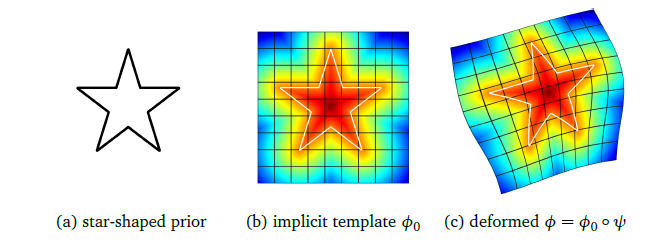
\includegraphics[width=\textwidth]{img_seg/implicit}
    \caption{Implicit template deformation: the segmentation corresponds to the deformed initial template. (Source:~\textcite{mory2011})}
    \label{fig:implicit}
\end{figure}

Once the deformation has been found through the minimization of Equation~\ref{eq:implicit}, the segmentation is obtained by applying it to the template, as illustrated in Figure~\ref{fig:implicit}.

%%%%%%%%%%%%%%%%%%%%%%%%%%%%%%%%%%%%%%%%%%%%%%%%%%%%%%%%%%%%%%%%%%%%%%%%%%%%%%%%%%%%%%%%%%%%%%%
\section{Template Deformation via Deep Learning}
\label{sec:deformable_dl}

The method presented in this section produces the segmentation of an image given said image and a fixed template. The deformation to be applied to the template is predicted by a neural network. Following the reasoning of~\textcite{mory2012MICCAI}, we define the deformation $\psi$ as the composition of a global transformation $G$ and a local transformation $L$: $\psi = G \circ L$.

\begin{figure}[htbp]
	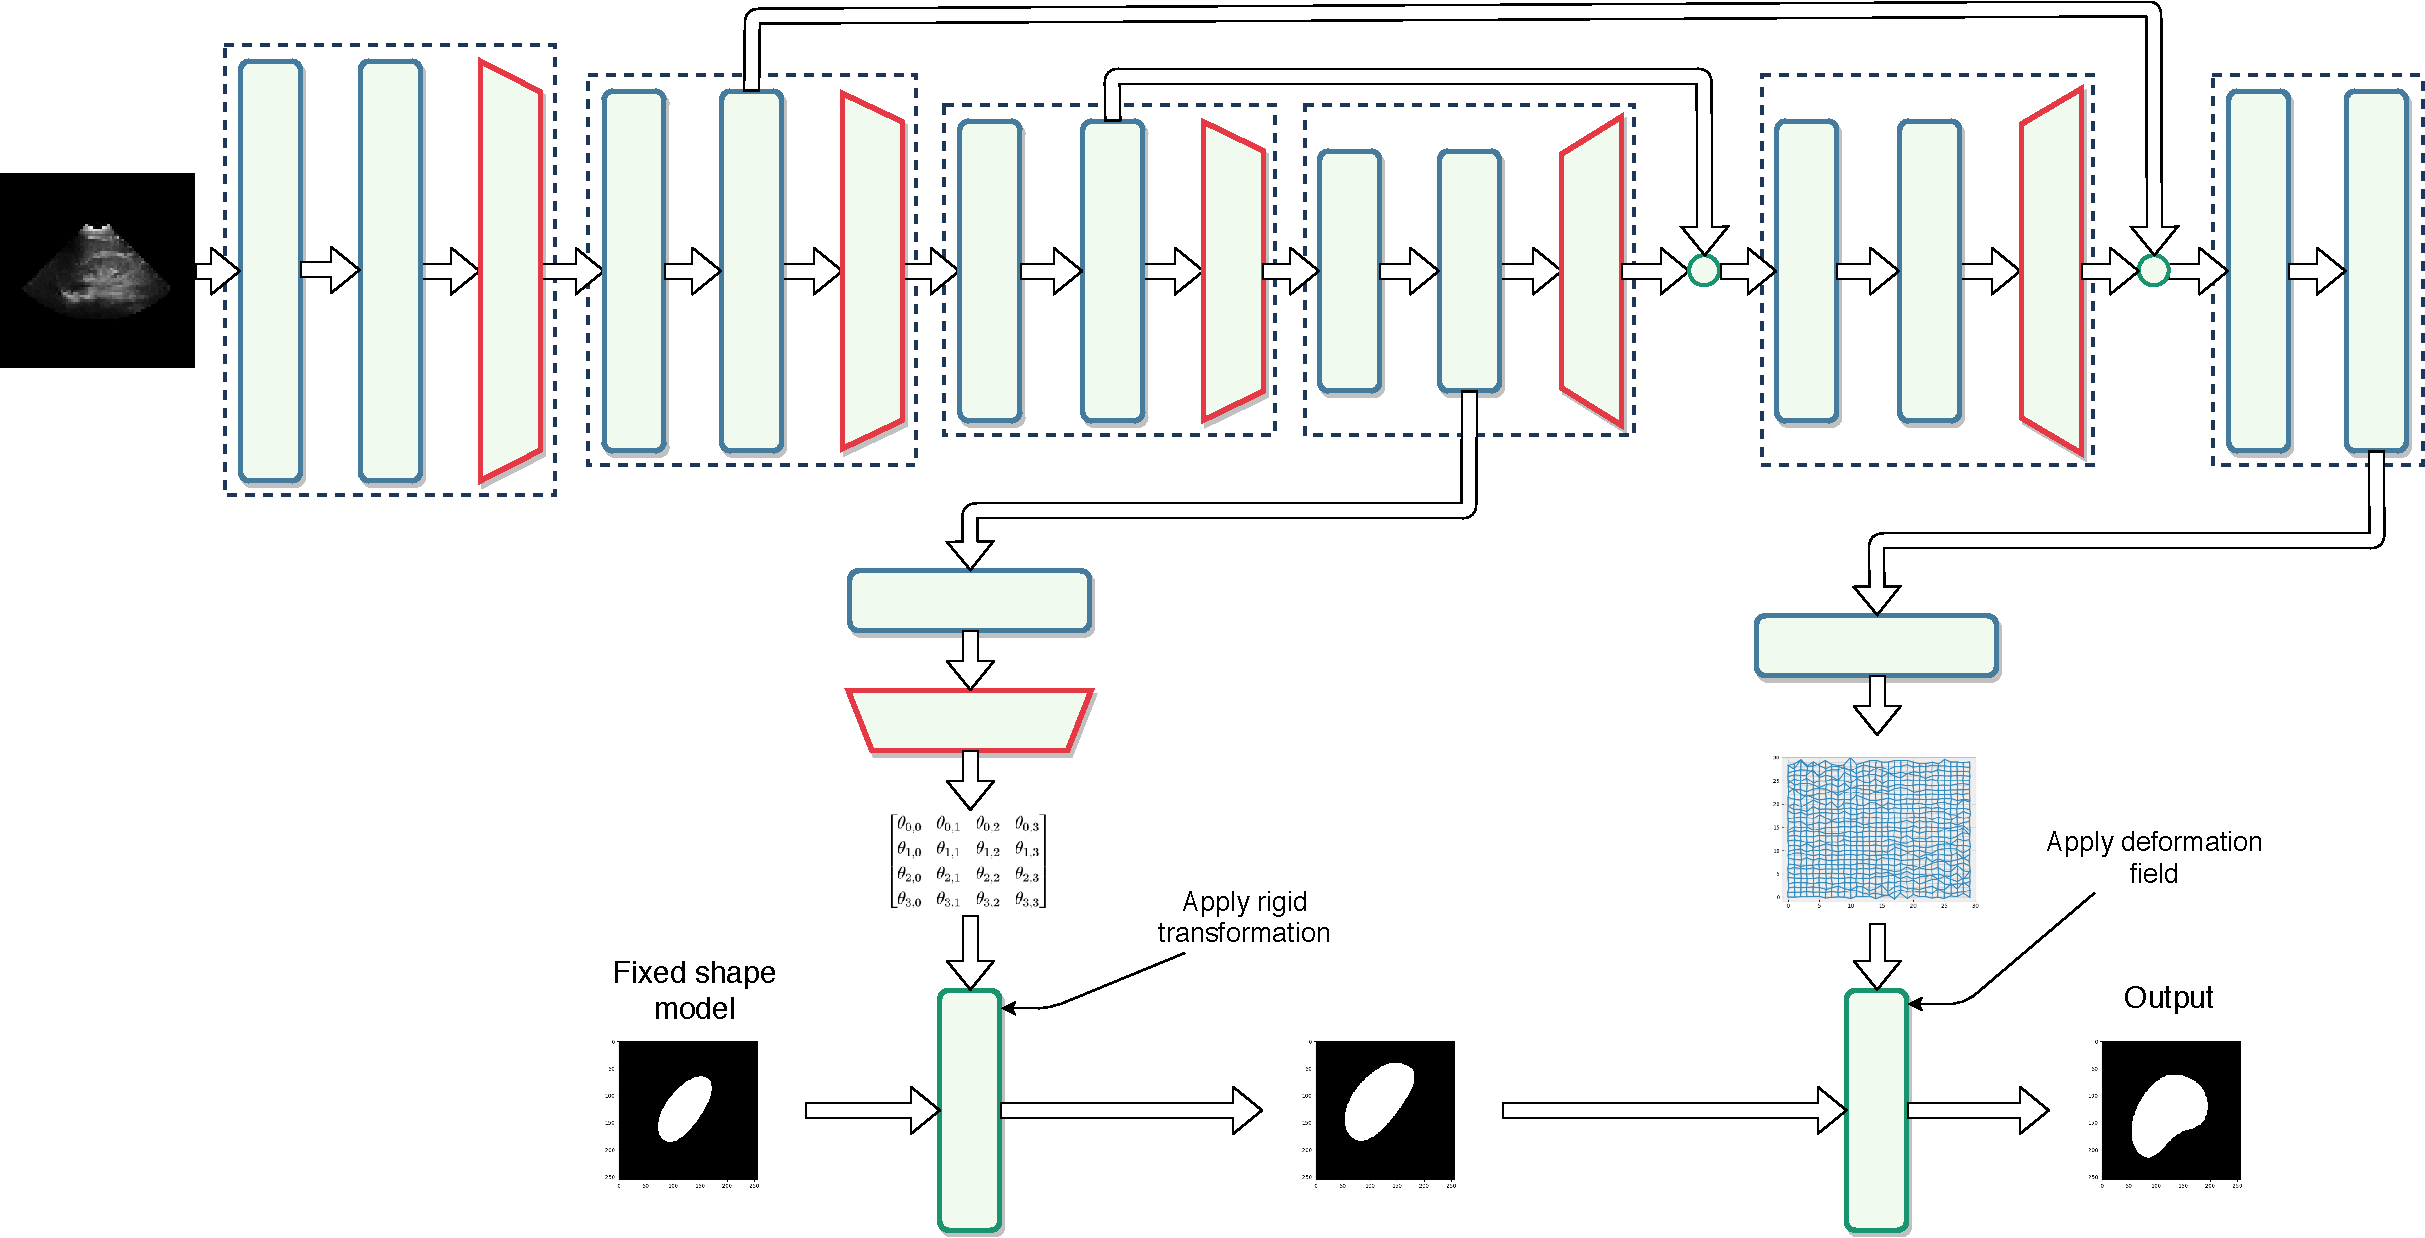
\includegraphics[width=\textwidth]{img_seg/deformation_network}
    \caption{Segmentation network that predicts a global geometric transformation and a deformation field to deform a template.}
    \label{fig:deform_network}
\end{figure}

Figure~\ref{fig:deform_network} shows the neural network. The network predict the global transformation $G$ and the local transformation $L$ from the image, which are then applied to the template $\phi_0$:

\begin{equation}
    \phi = \phi_0 \circ \ G \circ L
\end{equation}

The next sections details our choice of global transformation (Section~\ref{ssec:seg_global}), of local transformation (Section~\ref{ssec:seg_local}) and how to train the network (Section~\ref{ssec:seg_training}).

%%%%%%%%%%%%%%%%%%%%%%%%
\subsection{Global transformation}
\label{ssec:seg_global}

A geometric transformation for 3D images is represented by a $4 \times 4$ matrix, meaning a total of 16 parameters that can be predicted. Directly predicting those parameters remove control on the kind of transformation that are predicted. In our case, we chose to predict instead translation, rotation and scaling parameters. 

Three parameters are predicted for the translation on each axis, giving the following translation matrix $T$:
\begin{equation*}
    T = 
    \begin{bmatrix}
        1 & 0 & 0 & t_x \\
        0 & 1 & 0 & t_y \\
        0 & 0 & 1 & t_z \\ 
        0 & 0 & 0 & 1
    \end{bmatrix}
\end{equation*}

The scaling matrix $S$ is built from three more parameters:
\begin{equation*}
    S = 
    \begin{bmatrix}
        s_x & 0 & 0 & 0 \\
        0 & s_y & 0 & 0 \\
        0 & 0 & s_z & 0 \\ 
        0 & 0 & 0 & 1
    \end{bmatrix}
\end{equation*}

Finally, we have one rotation matrix in each direction ($R_x$, $R_y$ and $R_z$) built from one parameter each:
\begin{equation*}
    R_x = 
    \begin{bmatrix}
        1 & 0 & 0 & 0 \\
        0 & \cos{r_x} & -\sin{r_x} & 0 \\
        0 & \sin{r_x} & \cos{r_x} & 0 \\ 
        0 & 0 & 0 & 1
    \end{bmatrix}
\end{equation*}
\begin{equation*}
    R_y = 
    \begin{bmatrix}
        \cos{r_y} & 0 & - \sin{r_y} & 0 \\
        0 & 1 & 0 & 0 \\
        \sin{r_y} & 0 & \cos{r_y} & 0 \\ 
        0 & 0 & 0 & 1
    \end{bmatrix}
    \mkern20mu
    R_z = 
    \begin{bmatrix}
        \cos{r_z} & -\sin{r_z} & 0 & 0 \\
        \sin{r_z} & \cos{r_z} & 0 & 0 \\
        0 & 0 & 1 & 0 \\ 
        0 & 0 & 0 & 1
    \end{bmatrix}
\end{equation*}

We also need to center the image around zero before applying the rotations, which requires no parameters except knowing the center of the image:
\begin{equation*}
    C_+ = 
    \begin{bmatrix}
        1 & 0 & 0 & c_x \\
        0 & 0 & 0 & c_y \\
        0 & 0 & 0 & c_z \\ 
        0 & 0 & 0 & 1
    \end{bmatrix}
    \mkern20mu
    C_- = 
    \begin{bmatrix}
        1 & 0 & 0 & -c_x \\
        0 & 0 & 0 & -c_y \\
        0 & 0 & 0 & -c_z \\ 
        0 & 0 & 0 & 1
    \end{bmatrix}
\end{equation*}

From these matrices, the geometric transformation $G$ applied to the shape model is the following:
\begin{equation}
    G = T \cdot C_+ \cdot R_z \cdot R_y \cdot R_x \cdot S \cdot C_-
\end{equation}

The prediction of the 9 required parameters is done by a convolutional layer with 9 $1 \times 1 \times 1$ filters, followed by an average pooling layer of the size of the feature maps. 

%%%%%%%%%%%%%%%%%%%%%%%%
\subsection{Local deformation}
\label{ssec:seg_local}

The deformation field $v$ are predicted from a convolutional layer with 3 $3 \times 3 \times 3$ filters, one filter per dimension. Each field is then smoothed with a $3 \times 3 \times 3$ mean filter, before being resized to the shape model size with a tri-linear interpolation. This resizing step allows predicting deformation fields at a lower resolution than the shape model, saving time and parameters to learn.
\begin{equation}
    L = u(x) + Id = [K_{\sigma} * v](x) + Id
\end{equation}
As in the implicit template deformation case, the Gaussian filtering is there to enforce the regularity of the deformation field.

% We added an $L_2$ penalty term to the deformation fields $\psi$ in the loss function:
% \begin{equation}
%     P = \lambda \sum_x \left( L - Id \right)(x)^2
% \end{equation}
% $\lambda$ is the strength of this term, chosen as $10^{-3}$. The goal of this penalty term is to constrain the size of the deformation fields.

%%%%%%%%%%%%%%%%%%%%%%%%
\subsection{Training and loss function}
\label{ssec:seg_training}

Our segmentation method requires only the usual database of images and their ground-truth segmentation expressed as binary masks. For simplicity (and lack of time), the template is chosen as one of those segmentation. The corresponding image is then excluded from training and testing. 

Applying the global and local transformation to the template can be done as a layer of the network that outputs the final segmentation. As such, the loss function $J$ is simply the Dice coefficient between the network's output $\hat{\phi}$ and the ground-truth segmentation $\phi$:
\begin{align}
    J \left( \phi, \hat{\phi} \right) = DICE \left( \phi, \hat{\phi} \right)% + \frac{\lambda}{2} || L - Id ||^2_2 \\
                                      = DICE \left( \phi_0 \circ G \circ L, \hat{\phi} \right)% + \frac{\lambda}{2} || L - Id ||^2_2
\end{align}
The only free variables are $G$ and $L$, which are predicted by the network. Training the network as standard by backpropagation on a database of images allows it to predict $G$ and $L$ for new images. 

%%%%%%%%%%%%%%%%%%%%%%%%%%%%%%%%%%%%%%%%%%%%%%%%%%%%%%%%%%%%%%%%%%%%%%%%%%%%%%%%%%%%%%%%%%%%%%%
\section{Kidney Segmentation in 3D Ultrasound}
\label{sec:seg_data}

The problem addressed is the same as in Section~\ref{sec:kidney}: kidney capsule segmentation in 3D ultrasound data from potentially ill children. The difference is that we are not in a transfer learning setting and we have access to both adults and children images simultaneously.

While our new segmentation method is applicable to any kind of medical imaging segmentation problem, time constraint forced us to focus on an already available dataset. As the problem is difficult, this is still a good test of the method, though further testing is required. 

%%%%%%%%%%%%%%%%%%%%%%%%%%%%%%%%%%
%\subsection{Dataset}

\begin{figure}[htb]
        \begin{subfigure}[b]{0.245\textwidth}
                \centering
                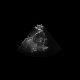
\includegraphics[width=\linewidth]{img_seg/30_post}
        \end{subfigure}%
        \hspace{1px}
        \begin{subfigure}[b]{0.245\textwidth}
                \centering
                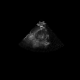
\includegraphics[width=\linewidth]{img_seg/32_post}
        \end{subfigure}%
        \begin{subfigure}[b]{0.245\textwidth}
                \centering
                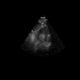
\includegraphics[width=\linewidth]{img_seg/33_post}
        \end{subfigure}%
        \begin{subfigure}[b]{0.245\textwidth}
                \centering
                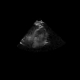
\includegraphics[width=\linewidth]{img_seg/37_post}
        \end{subfigure}
        
        \begin{subfigure}[b]{0.245\textwidth}
                \centering
                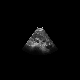
\includegraphics[width=\linewidth]{img_seg/70_post}
        \end{subfigure}%
        \hspace{1px}
        \begin{subfigure}[b]{0.245\textwidth}
                \centering
                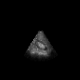
\includegraphics[width=\linewidth]{img_seg/71_post}
        \end{subfigure}%
        \begin{subfigure}[b]{0.245\textwidth}
                \centering
                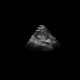
\includegraphics[width=\linewidth]{img_seg/72_post}
        \end{subfigure}%
        \begin{subfigure}[b]{0.245\textwidth}
                \centering
                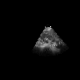
\includegraphics[width=\linewidth]{img_seg/75_post}
        \end{subfigure}
        
        \begin{subfigure}[b]{0.245\textwidth}
                \centering
                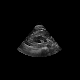
\includegraphics[width=\linewidth]{img_seg/280_post}
        \end{subfigure}%
        \hspace{1px}
        \begin{subfigure}[b]{0.245\textwidth}
                \centering
                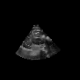
\includegraphics[width=\linewidth]{img_seg/282_post}
        \end{subfigure}%
        \begin{subfigure}[b]{0.245\textwidth}
                \centering
                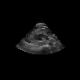
\includegraphics[width=\linewidth]{img_seg/286_post}
        \end{subfigure}%
        \begin{subfigure}[b]{0.245\textwidth}
                \centering
                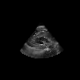
\includegraphics[width=\linewidth]{img_seg/288_post}
        \end{subfigure}
        \caption{Original images after pre-processing (left column) and augmented images (other three columns).}
        \label{fig:data_aug}
\end{figure}

The dataset stays identical as in Section~\ref{ssec:data}, as well as the pre-processing. We have 503 healthy adults images and 64 children. The images have been down-sampled to a resolution of $4 \times 4 \times 4$ mm$^3$, and centered in a $80 \times 80 \times 80$ voxels cube. 

\begin{table}[htb]
	\centering
	\begin{tabular}{|l|c|c|}
	    \hline
                        & Mean & Standard deviation \\
        \hline
         Gaussian noise & $0$ & $5$ \\
         Translation & $0$ & $3$ \\
         Rotation & $0$ & $0.05$ \\
         Scaling & $1$ & $0.05$ \\
        \hline
    \end{tabular}
	\caption{Data augmentation used for the kidney dataset. The parameters for each type of augmentation are drawn from a normal distribution with the mean and standard deviation specified.}
	\label{table:data_aug}
\end{table}

Unlike previously, we use data augmentation. Due to the already high cost of training on this dataset, each image is augmented 10 times before training. The augmentation includes adding Gaussian noise, as well as translation, rotation and scaling of the image (and the segmentation). The range of each type of augmentation is shown in Table~\ref{table:data_aug}. Some augmented images are shown in Figure~\ref{fig:data_aug} alongside their original image.

%%%%%%%%%%%%%%%%%%%%%%%%%%%%%%%%%%%%%%%%%%%%%%%%%%%%%%%%%%%%%%%%%%%%%%%%%%%%%%%%%%%%%%%%%%%%%%%
\section{Results and Discussion}
\label{sec:seg_result}

\begin{table}[htbp]
	\centering
\begin{tabular}{|l|c|c|c|c|}
	\hline
    Method & Dice Adults & Dice Children \\
	\hline
    3D U-Net & $\bm{0.89}$ & $\bm{0.82}$ \\
    Deformation & $0.85$ & $0.75$ \\
    Geometric transfo + Deformation & $0.88$ & $\bm{0.82}$ \\
    %Geometric transfo + Deformation + $L_2$ penalty & ??? & ??? \\
    \hline
\end{tabular}
	\vspace{2mm}
	\caption{Performance of the baseline and the shape model methods.}
    \label{table:seg_results}
\end{table}

For all the models the training is done jointly on adults and children with oversampling of the children to balance the populations. Each model was trained on only one seed due to the high cost of training (around five days per model). The performance of each model is reported in Table~\ref{table:seg_results}.

The baseline for our comparison is the 3D U-Net (\textcite{cicek2016MICCAI}) described in Section~\ref{ssec:unet}. Its performance is therefore comparable to the one reported in Section~\ref{sec:kidney_res}, the only difference being the use of data augmentation. The performance goes from $0.81$ for the adults and $0.74$ for the children to $0.89$ and $0.82$, an important increase of $0.08$ for both populations. 

Training a model predicting only deformation fields without the geometric transformation is not enough to beat the baseline, though it does show that the idea works. When adding the geometric transformation, the results become very close to the baseline. The geometric transformation is beneficial in particular for the children. This is likely due to the fact that the template model is an adult kidney, requiring the network to learn how to shrink it when segmenting children images. The geometric transformation provides an easy way to learn this shrinking with the three scaling parameters.

%[TODO penalty results]

% \begin{figure}[htbp]
%   \begin{subfigure}[b]{0.5\linewidth}
%     \centering
%     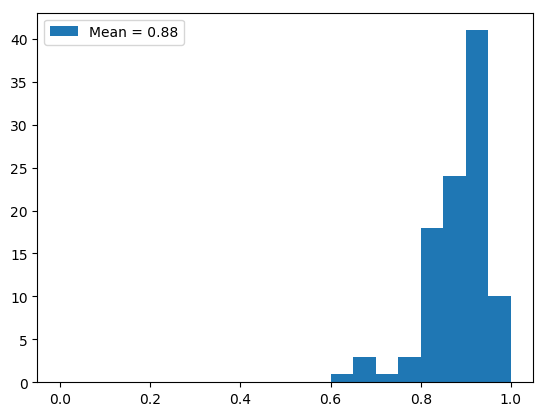
\includegraphics[width=0.95\linewidth]{img_seg/dice_hist_adults} 
%   \end{subfigure}%% 
%   \begin{subfigure}[b]{0.5\linewidth}
%     \centering
%     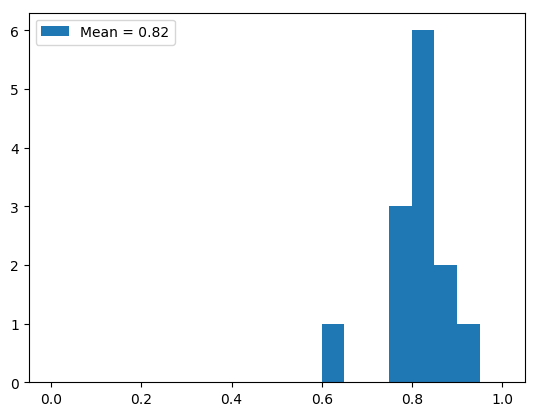
\includegraphics[width=0.95\linewidth]{img_seg/dice_hist_children} 
%   \end{subfigure} 
%   \caption{Histograms of Dice coefficient for the model with geometric transformation and deformation fields. Left: Dice coefficient on adults, right: Dice coefficient on children.}
%   \label{fig:seg_hist}
% \end{figure}

\begin{figure}[htbp]
    \centering
	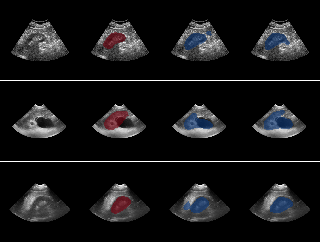
\includegraphics[width=\textwidth]{img_seg/unet_vs_deform}
    \caption{Comparing 3D U-Net results and deformation fields results. From left to right: image, ground truth, U-Net segmentation, deformation fields segmentation.}
    \label{fig:unet_vs_deform}
\end{figure}

Even though the performance of our method is similar to the baseline, using the template model results in segmentation anatomically correct. There are no patches of disconnected voxels classified as kidney or unlikely shapes. In Figure~\ref{fig:unet_vs_deform}, we selected three images from the test set to illustrate this. In the first one, the U-Net segmented a patch of pixel in the top left disconnected from the rest\footnote{As we show only a slice of a volume, the patch could be connected through the other slices, this is not the case here.}, while our method did not. The second image is difficult as the huge black spot can be mistaken for hydronephrosis. While both networks classified it as kidney, our method kept the elongated shape of the kidney outside of the black spot. In the third image, the U-Net segmented a patch of pixels almost disconnected from the main patch which would be very difficult to obtain by deforming a template model, as our method shows. 

\begin{figure}[htbp]
    \centering
	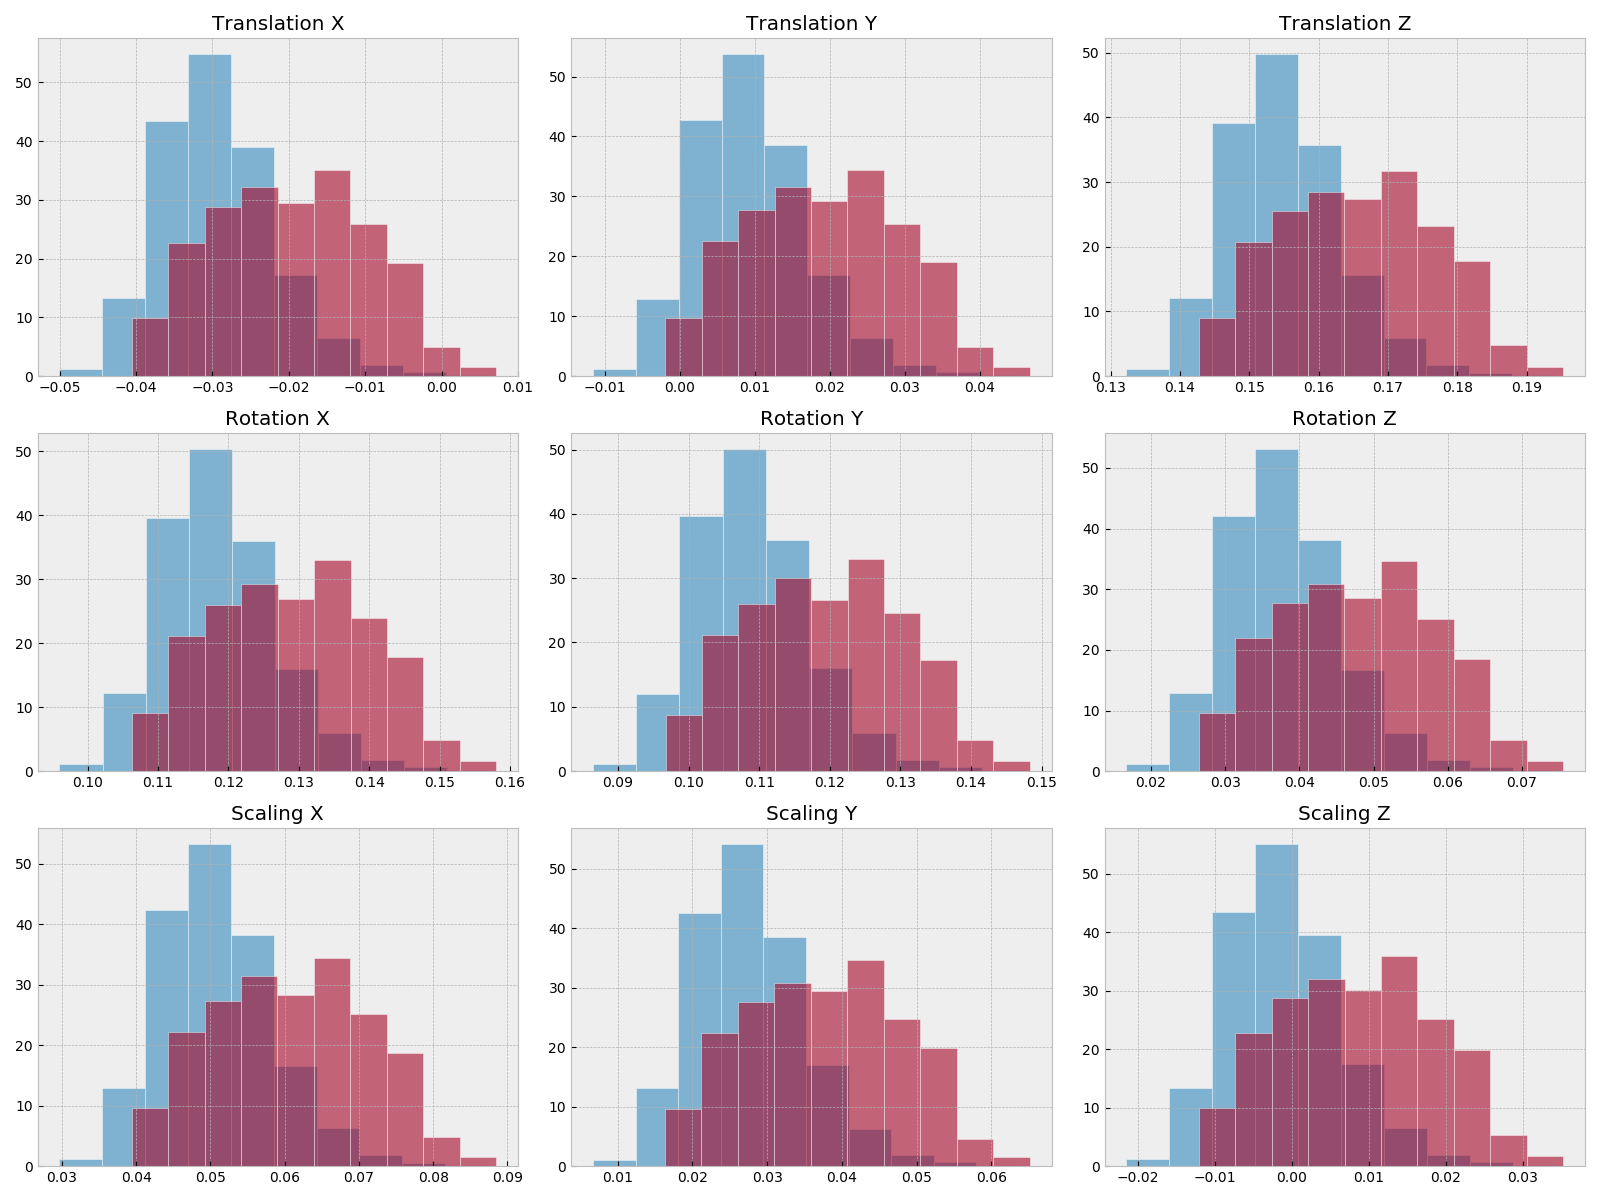
\includegraphics[width=\textwidth]{img_seg/transfo_matrix}
    \caption{Distributions of each parameter of the geometric transformation for the model without penalty. Red is for the adults, blue for the children.}
    \label{fig:transfo_matrix}
\end{figure}

Since the geometric transformation provided an important boost in performance, we look at the distribution of each parameter predicted on the test set in Figure~\ref{fig:transfo_matrix}. 

First we note that the distributions are almost identical for all parameters. Looking at the values for individual images reveals that the parameters are correlated, i.e. if a parameter falls on the lower side of the distribution for an image, the other parameters will also fall on the lower side of their distributions for the same image. This is likely due to using only one convolutional layer to predict the parameters, i.e. a lack of capacity.

The second point of interest is that the distributions between adults and children are very different. The children tends to have lower parameter values and the adults are spread out over a bigger range. This makes sense for the scaling parameters: as the template is based on an adult's kidney, it is necessary to shrink it more to match the size of a children. However there are no reasons why this should be true for the translation and rotation. This is possibly a side-effect of the parameters being so correlated. If the network lacked capacity, it make sense to focus on the most important parameters, the scaling, and the other followed.

Finally, looking at the actual value of the parameters, it seems that the network relies on a very specific transformation to work. Every parameter falls into a narrow range of values. For all images, the template is translated, rotated and scaled in roughly the same direction and amplitude. 

The very low values of the scaling means the template model is heavily shrunk. As a result, the deformation fields have very high values to match the target. %The goal of the $L_2$ penalty is to change this by penalizing high values for the deformation fields.

%[TODO why are high values bad ?]

%[TODO geometric transfo distributions for penalty model]

%%%%%%%%%%%%%%%%%%%%%%%%%%%%%%%%%%%%%%%%%%%%%%%%%%%%%%%%%%%%%%%%%%%%%%%%%%%%%%%%%%%%%%%%%%%%%%%
\section{Conclusion}

In this chapter we presented a new segmentation method based on template deformation via deep learning. This method does not require ground-truth deformation fields, but only the standard ground-truth segmentation masks. As such, it can be applied to any medical imaging segmentation problem where the use of a template makes sense.

As this work was done at the very end of the PhD, it is still incomplete, and there are some simple modifications that would likely improve the performance. 

To avoid the very low values of the scaling parameters, the solution is to add an $L_2$ regularization term to the deformation field $L$:
\begin{equation}
    \mathbf{R} \left( L \right) = \frac{\lambda}{2} \sum_x \left( L - Id \right)(x)^2
\end{equation}
This would strongly reduce the magnitude of the deformation fields and force the scaling into a more sensible range. 

To counter the strong correlation between the parameters of the global transformation, we should increase the capacity of the network by adding one or two convolutional layers just before the parameters prediction.

The other aspect of this work that merits attention is the choice of template. We chose the simplest method of simply using one of the ground-truth segmentation as the template, but more complex methods are likely to yield better results. In particular the work of~\textcite{prevost2013PHD} learns the mean shape and possible variations and integrates it into the implicit template deformation framework, making it a natural fit with our approach.
